\documentclass[a4paper,10pt]{article}
\usepackage[english]{babel}
\usepackage[utf8]{inputenc}
\usepackage{graphicx}
\usepackage{amsmath,amssymb}
\usepackage{hyperref, url}
\usepackage{listings}
\usepackage[multiple]{footmisc}
\usepackage[english]{babel}
\usepackage{float}
\parindent 0mm
\parskip 3mm

% add your name and student number in parenthesis
\title{ICS-E4020: Week 4 - Correlated pairs GPU}
\author{Néstor Castillo García (472081)\\ 
       {\tt nestor.castillogarcia@aalto.fi}}
\begin{document}

\maketitle

\section{Correlated pairs in GPU }

\subsection{Description}

Using CUDA, a working solution that solved the image correlation problem on the GPU was done.


\subsection{Hardware}
The computers had the following specifications: Intel Xeon E3-1230v2, 4 cores, 8 thread, 3,3 GHz, RAM: 16 GB, GPU: Nvidia K2000.

\subsection{Performance}
As the focus of this exercise was not in performance, it was not heavily optimised. Nevertheless, this GPU version did the correlated pairs task of a 4000 x 4000 image in less than 15s; faster than a double threaded version but slower than a 8-threaded version. The block size does matter in the performance, for this case the optimal block size was 8 x 8 threads as shown in figure 1. 

\begin{figure}[H]
\centering
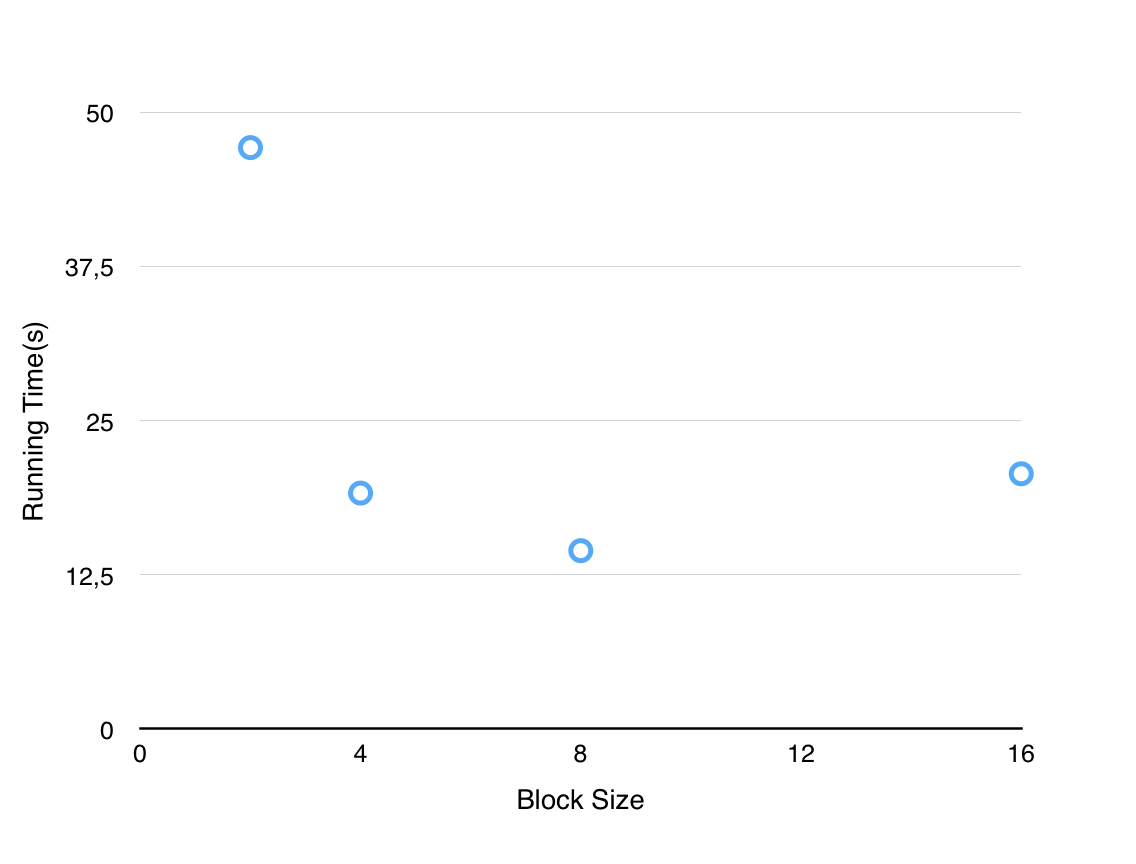
\includegraphics[width=1\textwidth]{figures/w4_timevsBlockSize}
\caption{Time vs BlockSize (squared) in a 4000 x 4000 image}
\label{fig:pca_type}
\end{figure}

\begin{figure}[H]
\centering
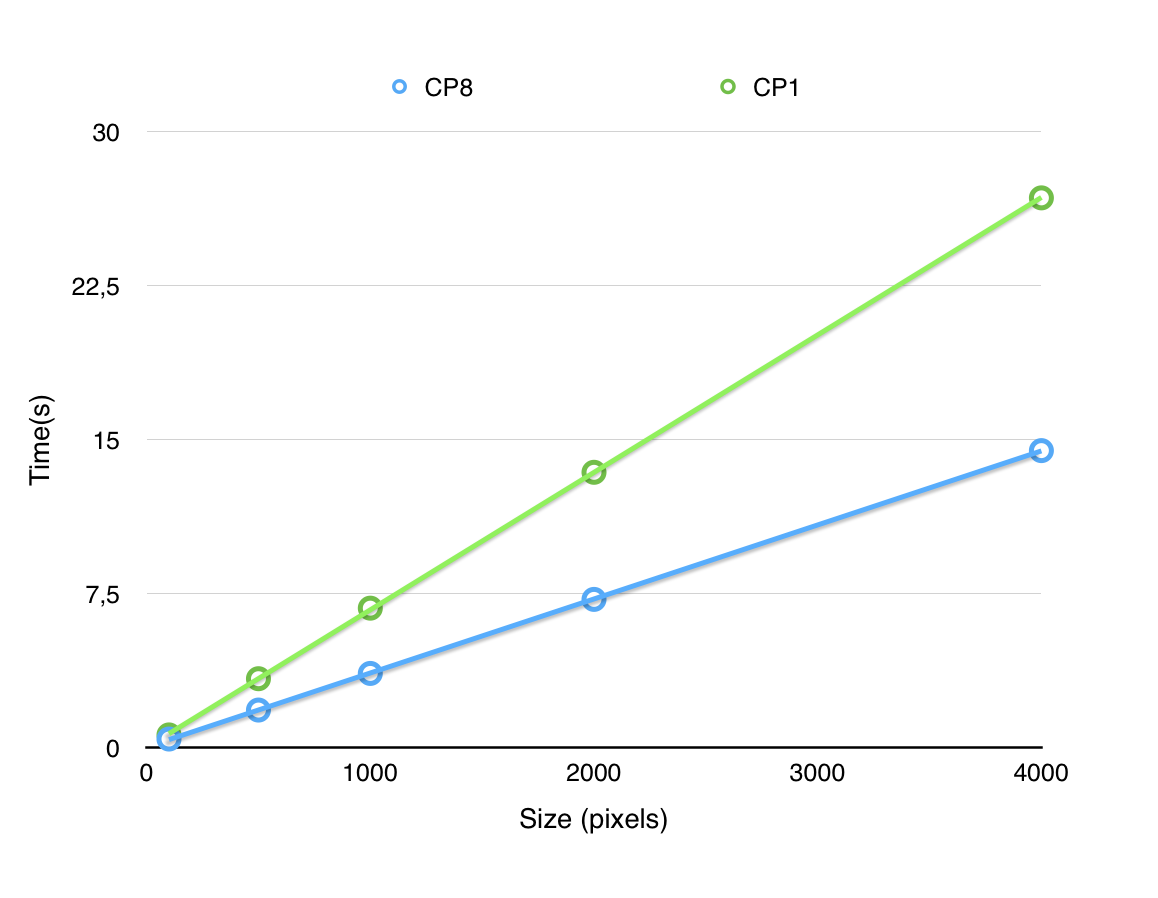
\includegraphics[width=1\textwidth]{figures/w4_cp1Vscp8}
\caption{Single threaded version vs GPU implementation in a 4000 * N image}
\label{fig:pca_type}
\end{figure}

\begin{figure}[H]
\centering
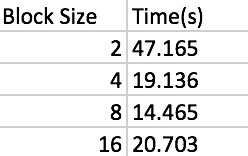
\includegraphics[width=0.5\textwidth]{figures/w4_blockSizeTable}
\caption{Time vs BlockSize table in a 4000 x 4000 image}
\label{fig:pca_type}
\end{figure}

The code was profiled with nvidia profiler and it was found that the kernel execution time occupies 98,8\% of the total time. Thus, the cudaMemCopy instructions occupy a small amount of time compared to the kernel execution. 

\begin{figure}[H]
\centering
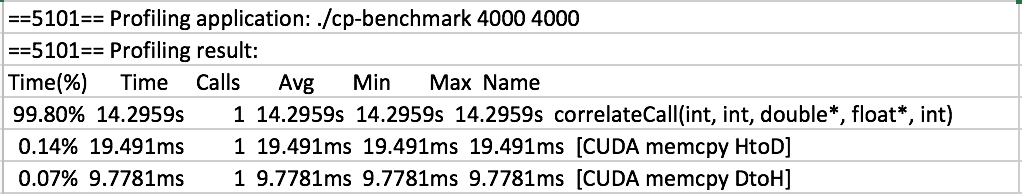
\includegraphics[width=0.1\textwidth]{figures/w4_timing}
\caption{Detailed execution time in a 4000 x 4000 image}
\label{fig:pca_type}
\end{figure}

\begin{figure}[H]
\centering
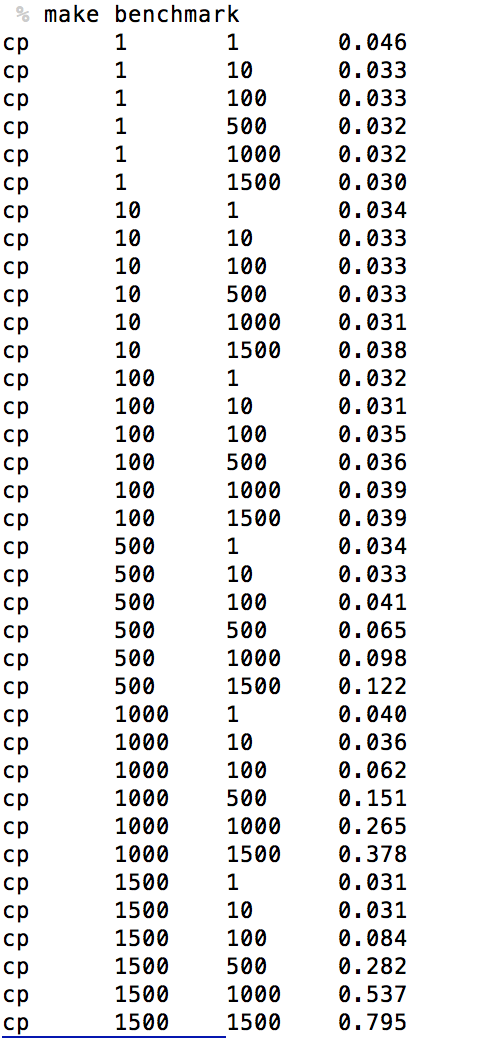
\includegraphics[width=0.5\textwidth]{figures/w4_benchmark}
\caption{Benchmark results}
\label{fig:pca_type}
\end{figure}




\subsection{So1 resubmission}
NOTE: My last submission of so1 was rejected due to a fail in make DEBUG=2. However, as stated in email conversations, it was due to a "compiler bug" so I was allowed to resumbit without losing points.  


I\end{document}